\documentclass[11pt,a4paper]{report}
\usepackage[textwidth=37em,vmargin=30mm]{geometry}
\usepackage{calc,xunicode,amsmath,amssymb,paralist,enumitem,tabu,booktabs,datetime2,xeCJK,xeCJKfntef,listings}
\usepackage{tocloft,fancyhdr,tcolorbox,xcolor,graphicx,eso-pic,xltxtra,xelatexemoji}

\newcommand{\envyear}[0]{2024}
\newcommand{\envdatestr}[0]{2024-10-21}
\newcommand{\envfinaldir}[0]{webdb/2024/20241021/final}

\usepackage[hidelinks]{hyperref}
\hypersetup{
    colorlinks=false,
    pdfpagemode=FullScreen,
    pdftitle={Web Digest - \envdatestr}
}

\setlength{\cftbeforechapskip}{10pt}
\renewcommand{\cftchapfont}{\rmfamily\bfseries\large\raggedright}
\setlength{\cftbeforesecskip}{2pt}
\renewcommand{\cftsecfont}{\sffamily\small\raggedright}

\setdefaultleftmargin{2em}{2em}{1em}{1em}{1em}{1em}

\usepackage{xeCJK,xeCJKfntef}
\xeCJKsetup{PunctStyle=plain,RubberPunctSkip=false,CJKglue=\strut\hskip 0pt plus 0.1em minus 0.05em,CJKecglue=\strut\hskip 0.22em plus 0.2em}
\XeTeXlinebreaklocale "zh"
\XeTeXlinebreakskip = 0pt


\setmainfont{Brygada 1918}
\setromanfont{Brygada 1918}
\setsansfont{IBM Plex Sans}
\setmonofont{JetBrains Mono NL}
\setCJKmainfont{Noto Serif CJK SC}
\setCJKromanfont{Noto Serif CJK SC}
\setCJKsansfont{Noto Sans CJK SC}
\setCJKmonofont{Noto Sans CJK SC}

\setlength{\parindent}{0pt}
\setlength{\parskip}{8pt}
\linespread{1.15}

\lstset{
	basicstyle=\ttfamily\footnotesize,
	numbersep=5pt,
	backgroundcolor=\color{black!5},
	showspaces=false,
	showstringspaces=false,
	showtabs=false,
	tabsize=2,
	captionpos=b,
	breaklines=true,
	breakatwhitespace=true,
	breakautoindent=true,
	linewidth=\textwidth
}






\newcommand{\coverpic}[2]{
    % argv: itemurl, authorname
    Cover photo by #2~~(\href{#1}{#1})
}
\newcommand{\makeheader}[0]{
    \begin{titlepage}
        % \newgeometry{hmargin=15mm,tmargin=21mm,bmargin=12mm}
        \begin{center}
            
            \rmfamily\scshape
            \fontspec{BaskervilleF}
            \fontspec{Old Standard}
            \fontsize{59pt}{70pt}\selectfont
            WEB\hfill DIGEST
            
            \vfill
            % \vskip 30pt
            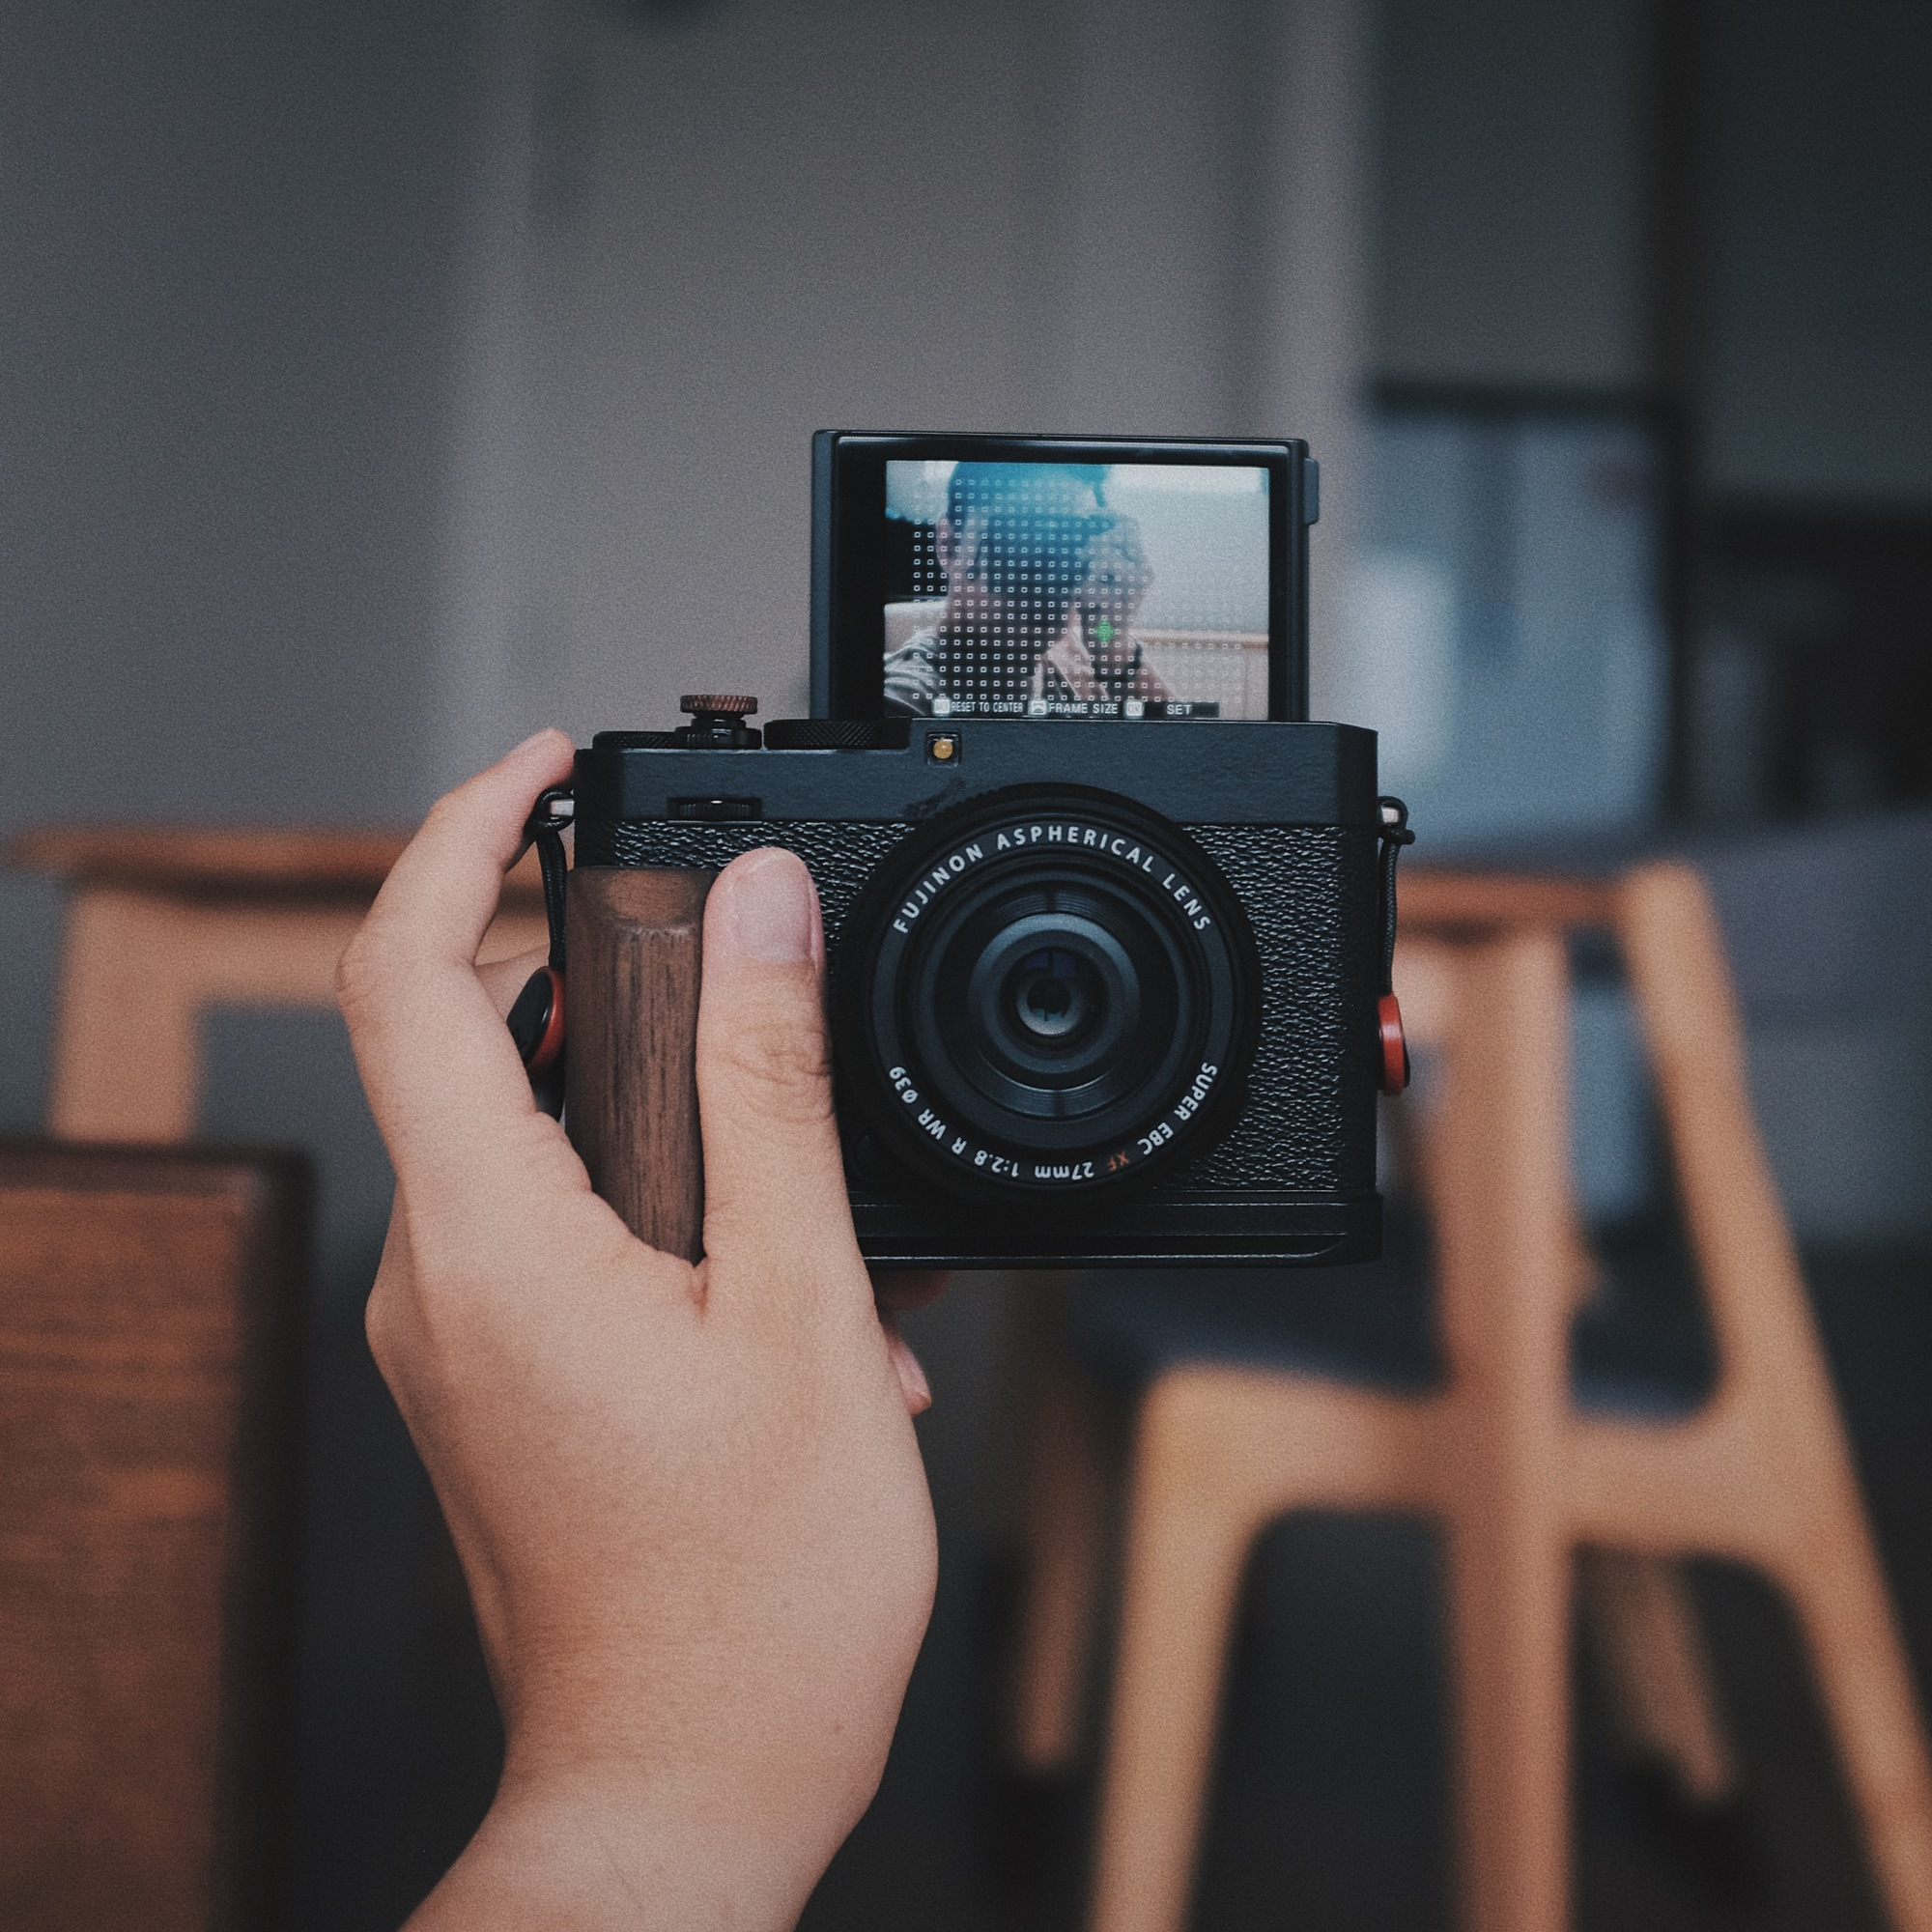
\includegraphics[width=\linewidth]{\envfinaldir/coverpic-prod.jpg}\par
            % \vskip 30pt
            \vfill

            \normalsize\rmfamily\scshape
            \copyright{} The Web Digest Project \hfill\large \envdatestr
        \end{center}
    \end{titlepage}
    % \restoregeometry
}
\newcommand{\simplehref}[1]{%
    \textcolor{blue!80!green}{\href{#1}{#1}}%
}
\renewcommand{\contentsname}{\center\Huge\sffamily\bfseries Contents\par\vskip 20pt}
\newcounter{ipartcounter}
\setcounter{ipartcounter}{0}
\newcommand{\ipart}[1]{
    % \vskip 20pt
    \clearpage
    \stepcounter{ipartcounter}
    \phantomsection
    \addcontentsline{toc}{chapter}{#1}
    % \begin{center}
    %     \Huge
    %     \sffamily\bfseries
    %     #1
    % \end{center}
    % \vskip 20pt plus 7pt
}
\newcounter{ichaptercounter}
\setcounter{ichaptercounter}{0}
\newcommand{\ichapter}[1]{
    % \vskip 20pt
    \clearpage
    \stepcounter{ichaptercounter}
    \phantomsection
    \addcontentsline{toc}{section}{\numberline{\arabic{ichaptercounter}}#1}
    \begin{center}
        \Huge
        \sffamily\bfseries
        #1
    \end{center}
    \vskip 20pt plus 7pt
}
\newcommand{\entrytitlefont}[1]{\subsection*{\raggedright\Large\sffamily\bfseries#1}}
\newcommand{\entryitemGeneric}[2]{
    % argv: title, url
    \parbox{\linewidth}{
        \entrytitlefont{#1}\par\vskip 5pt
        \footnotesize\ttfamily\mdseries
        \simplehref{#2}
    }\vskip 11pt plus 11pt minus 1pt
}
\newcommand{\entryitemGithub}[3]{
    % argv: title, url, desc
    \parbox{\linewidth}{
        \entrytitlefont{#1}\par\vskip 5pt
        \footnotesize\ttfamily\mdseries
        \simplehref{#2}\par\vskip 5pt
        \small\rmfamily\mdseries#3
    }\vskip 11pt plus 11pt minus 1pt
}
\newcommand{\entryitemAp}[3]{
    % argv: title, url, desc
    \parbox{\linewidth}{
        \entrytitlefont{#1}\par\vskip 5pt
        \footnotesize\ttfamily\mdseries
        \simplehref{#2}\par\vskip 5pt
        \small\rmfamily\mdseries#3
    }\vskip 11pt plus 11pt minus 1pt
}
\newcommand{\entryitemHackernews}[3]{
    % argv: title, hnurl, rawurl
    % \parbox{\linewidth}{
    %     \entrytitlefont{#1}\par\vskip 5pt
    %     \footnotesize\ttfamily\mdseries
    %     \simplehref{#3}\par
    %     \textcolor{black!50}{\href{#2}{#2}}
    % }\vskip 11pt plus 11pt minus 1pt
    \begin{minipage}{\linewidth}
            \entrytitlefont{#1}\par\vskip 5pt
            \footnotesize\ttfamily\mdseries
            \simplehref{#3}\par
            \textcolor{black!50}{\href{#2}{#2}}
    \end{minipage}\par\vskip 11pt plus 11pt minus 1pt
}







\begin{document}

\makeheader

\tableofcontents\clearpage




\ipart{Developers}
\ichapter{Hacker News}
\entryitemTwoLinks{WebGPU-Based WiFi Simulator}{https://news.ycombinator.com/item?id=41897214}{https://wifi-solver.com}

\entryitemTwoLinks{Kurt Vonnegut's lost board game published}{https://news.ycombinator.com/item?id=41896636}{https://www.polygon.com/board-games/467103/kurt-vonnegut-ghq-lost-board-game-publisher-interview}

\entryitemTwoLinks{Drasi: Microsoft's open source data processing platform for event-driven systems}{https://news.ycombinator.com/item?id=41896297}{https://github.com/drasi-project/drasi-platform}

\entryitemTwoLinks{The Part of PostgreSQL We Hate the Most (2023)}{https://news.ycombinator.com/item?id=41895951}{https://www.cs.cmu.edu/~pavlo/blog/2023/04/the-part-of-postgresql-we-hate-the-most.html}

\entryitemTwoLinks{Internet Archive breached again through stolen access tokens}{https://news.ycombinator.com/item?id=41895764}{https://www.bleepingcomputer.com/news/security/internet-archive-breached-again-through-stolen-access-tokens/}

\entryitemTwoLinks{The AI Investment Boom}{https://news.ycombinator.com/item?id=41895746}{https://www.apricitas.io/p/the-ai-investment-boom}

\entryitemTwoLinks{Syncthing Android App Discontinued}{https://news.ycombinator.com/item?id=41895718}{https://forum.syncthing.net/t/discontinuing-syncthing-android/23002}

\entryitemTwoLinks{Energy-based model explains how chronic stress transforms into disease over time}{https://news.ycombinator.com/item?id=41895609}{https://www.sciencedirect.com/science/article/pii/S030645302200292X}

\entryitemTwoLinks{How to do distributed locking (2016)}{https://news.ycombinator.com/item?id=41894451}{https://martin.kleppmann.com/2016/02/08/how-to-do-distributed-locking.html}

\entryitemTwoLinks{Using Euro coins as weights (2004)}{https://news.ycombinator.com/item?id=41894359}{https://www.rubinghscience.org/surv/euroweights1.html}

\entryitemTwoLinks{Bitwarden is no longer free software}{https://news.ycombinator.com/item?id=41893994}{https://github.com/bitwarden/clients/issues/11611}

\entryitemTwoLinks{The Best Darn Grid Shader (Yet) (2023)}{https://news.ycombinator.com/item?id=41893987}{https://bgolus.medium.com/the-best-darn-grid-shader-yet-727f9278b9d8}

\entryitemTwoLinks{Origin of 'Daemon' in Computing}{https://news.ycombinator.com/item?id=41891953}{https://www.takeourword.com/TOW146/page4.html}

\entryitemTwoLinks{Regarding our Cease and Desist letter to Automattic}{https://news.ycombinator.com/item?id=41891799}{https://wpfusion.com/business/regarding-our-cease-and-desist-letter-to-automattic/}

\entryitemTwoLinks{Accountability sinks}{https://news.ycombinator.com/item?id=41891694}{https://aworkinglibrary.com/writing/accountability-sinks}

\entryitemTwoLinks{QUIC is not quick enough over fast internet}{https://news.ycombinator.com/item?id=41890784}{https://arxiv.org/abs/2310.09423}

\entryitemTwoLinks{Show HN: I made a site to quick identify any plant and learn how to care for it}{https://news.ycombinator.com/item?id=41890762}{https://frondly.app/}

\entryitemTwoLinks{Italy's Piracy Shield just blocked one of Google's CDN}{https://news.ycombinator.com/item?id=41890460}{https://mil04s43-in-f1.1e100.net}

\entryitemTwoLinks{The Languages of English, Math, and Programming}{https://news.ycombinator.com/item?id=41890158}{https://github.com/norvig/pytudes/blob/main/ipynb/Triplets.ipynb}

\entryitemTwoLinks{Autism's Four Core Subtypes}{https://news.ycombinator.com/item?id=41889990}{https://www.thetransmitter.org/spectrum/untangling-biological-threads-from-autisms-phenotypic-patchwork-reveals-four-core-subtypes/}\ichapter{Phoronix}
\entryitemGeneric{\hskip 0pt{}Linux 6.12-rc4 Released With MSI Claw A1M Controller Support, Intel \& AMD Fixes}{https://www.phoronix.com/news/Linux-6.12-rc4-Released}

\entryitemGeneric{\hskip 0pt{}Intel Posts Patch For Fixing/Boosting Lunar Lake Linux Performance On ASUS Laptops}{https://www.phoronix.com/news/Intel-Lunar-Lake-ASUS-AIPT}

\entryitemGeneric{\hskip 0pt{}Concerns Raised Over Bitwarden Moving Further Away From Open-Source}{https://www.phoronix.com/news/Bitwarden-Open-Source-Concerns}

\entryitemGeneric{\hskip 0pt{}ReiserFS File-System Expected To Be Removed With Linux 6.13}{https://www.phoronix.com/news/Linux-6.13-To-Drop-ReiserFS}

\entryitemGeneric{\hskip 0pt{}Lightweight Guard Pages For Linux Showing 5x Speed-Up For Memory Mapping Invocations}{https://www.phoronix.com/news/Linux-Lightweight-Guard-Pages}

\entryitemGeneric{\hskip 0pt{}Audio Firmware Upstreamed For Qualcomm Snapdragon X1 On Linux}{https://www.phoronix.com/news/Linux-Snapdragon-X1-Audio-FW}

\entryitemGeneric{\hskip 0pt{}"100\% Free" GNU Boot Discovers Again They Have Been Shipping Non-Free Code}{https://www.phoronix.com/news/GNU-Boot-Second-Fail}

\entryitemGeneric{\hskip 0pt{}GNOME Making Progress On Full-Featured USB Portal For Flatpaks}{https://www.phoronix.com/news/GNOME-USB-Flatpaks-Portal}

\entryitemGeneric{\hskip 0pt{}Wine-Staging 9.20 Fixes An 11 Year Old Wine Bug Report}{https://www.phoronix.com/news/Wine-Staging-9.20}


\ipart{Developers~~~~(zh-Hans)}
\ichapter{Solidot}
\entryitemGeneric{\hskip 0pt{}82 岁老妇仍然骑 13 岁时父母送的自行车}{https://www.solidot.org/story?sid=79539}

\entryitemGeneric{\hskip 0pt{}德国主权科技基金过去两年向开源项目资助了逾  2300 万欧元}{https://www.solidot.org/story?sid=79538}

\entryitemGeneric{\hskip 0pt{}OpenAI 相对于其它 AI 公司的优势基本消失}{https://www.solidot.org/story?sid=79537}

\entryitemGeneric{\hskip 0pt{}古巴电网故障导致千万人断电}{https://www.solidot.org/story?sid=79536}

\entryitemGeneric{\hskip 0pt{}美国越来越多的父母拒绝给孩子接种疫苗}{https://www.solidot.org/story?sid=79535}

\entryitemGeneric{\hskip 0pt{}亚马逊高管告诉员工如果不喜欢强制重返办公室政策他们可以辞职}{https://www.solidot.org/story?sid=79534}

\entryitemGeneric{\hskip 0pt{}人类的嗅觉反应十分迅速}{https://www.solidot.org/story?sid=79533}

\entryitemGeneric{\hskip 0pt{}OpenAI 和微软的紧密关系出现裂缝}{https://www.solidot.org/story?sid=79532}

\entryitemGeneric{\hskip 0pt{}Gliese 229 B 被发现是一对棕矮星}{https://www.solidot.org/story?sid=79531}

\entryitemGeneric{\hskip 0pt{}高中生因使用 AI 受罚,其父母随后起诉教师和校长}{https://www.solidot.org/story?sid=79530}

\entryitemGeneric{\hskip 0pt{}新疗法能消除 2 型糖尿病患者对胰岛素的需求}{https://www.solidot.org/story?sid=79529}

\entryitemGeneric{\hskip 0pt{}欧盟考虑将马斯克其他公司的收入纳入 X 的潜在罚款计算内}{https://www.solidot.org/story?sid=79528}

\entryitemGeneric{\hskip 0pt{}NASA 冻结波音 Starliner 任务}{https://www.solidot.org/story?sid=79527}

\entryitemGeneric{\hskip 0pt{}香港诈骗集团用 AI 深度伪造欺骗受害者}{https://www.solidot.org/story?sid=79526}

\entryitemGeneric{\hskip 0pt{}Meta 解雇了 20 多名用餐券购买家庭用品的员工}{https://www.solidot.org/story?sid=79525}\ichapter{V2EX}
\entryitemGeneric{\hskip 0pt{}[宽带症候群] 日本闲置公网 IP 能干嘛}{https://www.v2ex.com/t/1082029}

\entryitemGeneric{\hskip 0pt{}[服务器] 使用 windows 的远程桌面, 链接到 Windows Server 2022 Datacenter 时, 最方便的多因素认证,是哪种方式?}{https://www.v2ex.com/t/1082028}

\entryitemGeneric{\hskip 0pt{}[Twitter] 推特锁区了如何支付?}{https://www.v2ex.com/t/1082027}

\entryitemGeneric{\hskip 0pt{}[宽带症候群] 检测到 NAT64。IPv6 工作,此问题如何解决?}{https://www.v2ex.com/t/1082026}

\entryitemGeneric{\hskip 0pt{}[Apple] 这价格入 MacBook Air M3 16+512 算好价吗?}{https://www.v2ex.com/t/1082024}

\entryitemGeneric{\hskip 0pt{}[宽带症候群] 2024 年了,帧中继(Frame Relay)现在还有提供商在使用吗?}{https://www.v2ex.com/t/1082023}

\entryitemGeneric{\hskip 0pt{}[程序员] QPS 到 3000 了,大家合理使用}{https://www.v2ex.com/t/1082022}

\entryitemGeneric{\hskip 0pt{}[程序员] 最近被空闲时间搞的有所困惑. 不知道如何合理利用空闲时间了. 睡不着, 一起聊聊.}{https://www.v2ex.com/t/1082021}

\entryitemGeneric{\hskip 0pt{}[问与答] 如何改善打开一堆 Chrome 窗口,每个窗口无数标签页的情况呢?}{https://www.v2ex.com/t/1082020}

\entryitemGeneric{\hskip 0pt{}[问与答] 失业后,进入了注册地为香港的公司,还能不能领取失业金}{https://www.v2ex.com/t/1082018}

\entryitemGeneric{\hskip 0pt{}[健康] 远房表妹 17 岁贫血,怎么办啊,各位前辈过来人支个招呗}{https://www.v2ex.com/t/1082015}

\entryitemGeneric{\hskip 0pt{}[生活] pc 的 web 端没有价值了么?}{https://www.v2ex.com/t/1082014}

\entryitemGeneric{\hskip 0pt{}[程序员] 求个思路:判断两个及以上的图形是否重叠。}{https://www.v2ex.com/t/1082013}

\entryitemGeneric{\hskip 0pt{}[生活] 关于坐车回家}{https://www.v2ex.com/t/1082012}

\entryitemGeneric{\hskip 0pt{}[分享发现] 日本签证政策发生变化了吗?}{https://www.v2ex.com/t/1082011}

\entryitemGeneric{\hskip 0pt{}[PayPal] Paypal 风控与人脸识别}{https://www.v2ex.com/t/1082010}

\entryitemGeneric{\hskip 0pt{}[求职] [求职]Rust 编程远程办公工作}{https://www.v2ex.com/t/1082009}

\entryitemGeneric{\hskip 0pt{}[程序员] 蹭热度:分析了一下这两天比较火的字节跳动实习生大模型训练集群投毒用到的漏洞的原理}{https://www.v2ex.com/t/1082008}

\entryitemGeneric{\hskip 0pt{}[iPhone] 美版有锁 + t mobile 是不是一个解?}{https://www.v2ex.com/t/1082007}

\entryitemGeneric{\hskip 0pt{}[NAS] 请问黑群晖硬盘数据怎么迁移到 unraid?}{https://www.v2ex.com/t/1082006}

\entryitemGeneric{\hskip 0pt{}[京东] 看到京东客服骂人``出生东西'',路转黑了}{https://www.v2ex.com/t/1082005}

\entryitemGeneric{\hskip 0pt{}[生活] 分享一下角膜移植后续斜视矫正经历}{https://www.v2ex.com/t/1082002}

\entryitemGeneric{\hskip 0pt{}[New York] 最近做了个方便找 hacker news 纯远程工作(国内|美国|欧洲)的网站}{https://www.v2ex.com/t/1082001}

\entryitemGeneric{\hskip 0pt{}[San Francisco] not just another hnhiring}{https://www.v2ex.com/t/1081998}

\entryitemGeneric{\hskip 0pt{}[问与答] 双十一 4k 显示器推荐}{https://www.v2ex.com/t/1081997}

\entryitemGeneric{\hskip 0pt{}[iPhone] 马上双 11 了,各位牛逼得 V 友,买 iPhone 16pro 512G 哪里最优惠}{https://www.v2ex.com/t/1081995}

\entryitemGeneric{\hskip 0pt{}[问与答] 有没有在香港做机房服务器托管的兄弟?来业务了。}{https://www.v2ex.com/t/1081994}

\entryitemGeneric{\hskip 0pt{}[问与答] Chrome 密码管理工具安全吗}{https://www.v2ex.com/t/1081991}

\entryitemGeneric{\hskip 0pt{}[问与答] 大家怎么看金砖支付系统 10 月 24 号上线}{https://www.v2ex.com/t/1081990}

\entryitemGeneric{\hskip 0pt{}[问与答] POTplayer 视频播放器去哪里下载比较好?}{https://www.v2ex.com/t/1081989}

\entryitemGeneric{\hskip 0pt{}[职场话题] 可能陷入了职场斗争之中该怎么处理}{https://www.v2ex.com/t/1081988}

\entryitemGeneric{\hskip 0pt{}[生活] 请大家帮忙分析下,这部分房价亏损的是谁的钱?}{https://www.v2ex.com/t/1081987}

\entryitemGeneric{\hskip 0pt{}[信息安全] 朋友手机被偷了,收到了钓鱼短信,有没有大佬给他一点教训}{https://www.v2ex.com/t/1081986}

\entryitemGeneric{\hskip 0pt{}[问与答] 有没有哪个网页可以直接体验下国内绿厂 OPPO color os、蓝厂 vivo 的 origin os、小米 HyperOS、华为的 harmony os}{https://www.v2ex.com/t/1081985}

\entryitemGeneric{\hskip 0pt{}[Apple] 有必要为了 Apple Intelligence 买港版 16 吗?}{https://www.v2ex.com/t/1081983}

\entryitemGeneric{\hskip 0pt{}[Windows] 垃圾 win11}{https://www.v2ex.com/t/1081982}

\entryitemGeneric{\hskip 0pt{}[iPhone] iPhone 升级换代,该考虑 512G 还是 1TB?}{https://www.v2ex.com/t/1081981}

\entryitemGeneric{\hskip 0pt{}[分享创造] [独立开发]捣鼓了一个健身 App,上架半年下载量只有两位数。。}{https://www.v2ex.com/t/1081980}

\entryitemGeneric{\hskip 0pt{}[分享创造] 闲来无事,做了一个小程序:有物记-你的个人物品管理专家!}{https://www.v2ex.com/t/1081979}

\entryitemGeneric{\hskip 0pt{}[视频技术] 开 emby 服的话需要先切片吗?}{https://www.v2ex.com/t/1081975}

\entryitemGeneric{\hskip 0pt{}[问与答] 记录一次交通事故的过程,还想问一下你们面对这种无赖到底是妥协还是出口恶气?}{https://www.v2ex.com/t/1081974}

\entryitemGeneric{\hskip 0pt{}[Node.js] 在设计一个 node 的插件化框架,学习 obsidian 插件但是有一些代码没看懂,请指教}{https://www.v2ex.com/t/1081973}

\entryitemGeneric{\hskip 0pt{}[问与答] 离婚可以提取住房公积金}{https://www.v2ex.com/t/1081971}

\entryitemGeneric{\hskip 0pt{}[问与答] 居民医保报销后,剩余自费部分可以用职工医保的个人账户支付吗?}{https://www.v2ex.com/t/1081969}

\entryitemGeneric{\hskip 0pt{}[Linux] 请问类似实验楼 www.shiyanlou.com(现在叫蓝桥云)中在线 Linux 平台如何实现的}{https://www.v2ex.com/t/1081968}

\entryitemGeneric{\hskip 0pt{}[iPad] 新版 iPad mini 的国行 esim 问题}{https://www.v2ex.com/t/1081967}

\entryitemGeneric{\hskip 0pt{}[问与答] 子网掩码 255.255.224.224 表示网络位有多少位?}{https://www.v2ex.com/t/1081965}

\entryitemGeneric{\hskip 0pt{}[游戏] Surface 现在还是 GALGAME 最佳游戏设备吗?}{https://www.v2ex.com/t/1081962}

\entryitemGeneric{\hskip 0pt{}[分享发现] 哈利路亚英文输入法功能比较完整地移植到 Windows 平台上了}{https://www.v2ex.com/t/1081961}

\entryitemGeneric{\hskip 0pt{}[问与答] 瘦客户机搞软路由确有性价比吗?}{https://www.v2ex.com/t/1081960}


\ipart{Generic News}
\ichapter{AP News}
\entryitemWithDescription{\hskip 0pt{}Lawyers for Sean `Diddy' Combs ask judge to release identities of his accusers}{https://apnews.com/article/1a6c2d9a44b1af2167322e9f3a13ec54}{}\ichapter{Reuters}
\entryitemWithDescription{\hskip 0pt{}Brazil's Lula cancels trip to BRICS summit on medical advice}{https://www.reuters.com/world/americas/brazils-lula-cancels-trip-brics-summit-kazan-medical-advice-2024-10-20/}{Brazilian President Luiz Inacio Lula da Silva on Sunday canceled his trip to Russia for the BRICS summit, following medical advice to temporarily avoid long-haul flights after hurting his head in an accident at...}

\entryitemWithDescription{\hskip 0pt{}Ukraine attacks forced Black Sea Fleet to move warships from Sevastopol, Russian official says}{https://www.reuters.com/world/europe/ukraine-attacks-forced-black-sea-fleet-move-warships-sevastopol-russian-official-2024-10-20/}{Russia\textquotesingle s Black Sea Fleet has been forced to move many warships from the naval base of Sevastopol on the Crimean peninsular, which Russia annexed in 2014, due to attacks by Ukraine, a Russian-installed official was quoted...}

\entryitemWithDescription{\hskip 0pt{}Thousands protest in Spain's Canary Islands against over tourism}{https://www.reuters.com/world/europe/thousands-protest-spains-canary-islands-against-over-tourism-2024-10-20/}{Thousands of people protested in holiday resorts in Spain\textquotesingle s Canary Islands on Sunday against over tourism which they say prices local people out of the housing...}

\entryitemWithDescription{\hskip 0pt{}Trudeau has wrecked Canada-India political relations, says expelled envoy}{https://www.reuters.com/world/trudeau-has-wrecked-canada-india-political-relations-says-expelled-envoy-2024-10-20/}{India\textquotesingle s envoy to Canada, who is being expelled over what Ottawa says are links to the murder of a Sikh leader, insisted in an interview he was innocent and said Prime Minister Justin Trudeau had wrecked bilateral political...}

\entryitemWithDescription{\hskip 0pt{}Serbia's Vucic thanks Putin for natural gas supplies}{https://www.reuters.com/world/europe/serbias-vucic-thanks-putin-natural-gas-supplies-2024-10-20/}{Serbian President Aleksandar Vucic said he thanked Russian President Vladimir Putin on Sunday for helping his country secure sufficient supplies of natural gas for the...}

\entryitemWithDescription{\hskip 0pt{}Senior Tanzanian opposition party official abducted and seriously injured, party says}{https://www.reuters.com/world/africa/senior-tanzanian-opposition-party-official-abducted-seriously-injured-party-says-2024-10-20/}{Unidentified people abducted, beat and seriously injured a senior Tanzanian opposition party official before dumping her in a forest, her party said on Sunday, a month after a similar abduction and murder of another of its party...}

\entryitemWithDescription{\hskip 0pt{}Kenya's impeached deputy president says his security withdrawn, safety at risk}{https://www.reuters.com/world/africa/kenyas-impeached-deputy-president-says-his-security-withdrawn-safety-risk-2024-10-20/}{The charges, which Rigathi Gachagua denies, included gross violation of the constitution and stirring ethnic...}

\entryitemWithDescription{\hskip 0pt{}Israel to take legal action against Macron over naval trade show ban}{https://www.reuters.com/world/israel-take-legal-action-against-macron-over-naval-trade-show-ban-2024-10-20/}{Israeli Foreign Minister Israel Katz said on Sunday he had ordered his ministry to start legal proceedings against French President Emmanuel Macron after Paris banned Israeli firms from participating in an upcoming military naval trade...}

\entryitemWithDescription{\hskip 0pt{}US investigates leak on intelligence about Israel's Iran attack plans}{https://www.reuters.com/world/us/investigation-underway-into-leak-us-intelligence-israel-iran-houses-johnson-says-2024-10-20/}{The United States is investigating the leak of a pair of highly classified intelligence documents describing Israel\textquotesingle s preparations for a retaliatory strike on Iran, House Speaker Mike Johnson said on...}

\entryitemWithDescription{\hskip 0pt{}Israel intensifies offensive in Gaza, Lebanon after Hamas leader's death}{https://www.reuters.com/world/middle-east/israel-intensifies-offensive-gaza-lebanon-after-hamas-leaders-death-2024-10-20/}{With U.S. elections approaching, officials, diplomats and other sources in the region say Israel is seeking to shield its borders and ensure its rivals cannot...}

\entryitemWithDescription{\hskip 0pt{}No clear winner in British Columbia election, with most votes counted}{https://www.reuters.com/world/americas/no-clear-winner-british-columbia-election-with-most-votes-counted-2024-10-20/}{The Canadian Broadcasting Corp said the result could depend on out-of-district votes and mail-in...}

\entryitemWithDescription{\hskip 0pt{}Gaza health ministry says 87 killed in northern Gaza airstrike}{https://www.reuters.com/world/middle-east/gaza-health-ministry-says-87-killed-northern-gaza-airstrike-2024-10-20/}{The incident in Beit Lahiya left one of the highest casualty tolls in...}

\entryitemWithDescription{\hskip 0pt{}'Everything is lost': Senegal repatriates citizens escaping Lebanon}{https://www.reuters.com/world/everything-is-lost-says-father-senegal-repatriates-citizens-escaping-lebanon-2024-10-20/}{"Ten minutes later, they called me: \textquotesingle there\textquotesingle s no more house, no more son...}






\clearpage
\leavevmode\vfill
\footnotesize

Copyright \copyright{} 2023-2024 Neruthes and other contributors.

This document is published with CC BY-NC-ND 4.0 license.

The entries listed in this newsletter may be copyrighted by their respective creators.

This newsletter is generated by the Web Digest project.

The newsletters are also delivered via Telegram channel \CJKunderline{\href{https://t.me/webdigestchannel}{https://t.me/webdigestchannel}}.\\
RSS feed is available at \CJKunderline{\href{https://webdigest.pages.dev/rss.xml}{https://webdigest.pages.dev/rss.xml}}.

This newsletter is available in PDF at
\CJKunderline{\href{https://webdigest.pages.dev/}{https://webdigest.pages.dev/}}.

The source code being used to generate this newsletter is available at\\
\CJKunderline{\href{https://github.com/neruthes/webdigest}{https://github.com/neruthes/webdigest}}.

This newsletter is also available in
\CJKunderline{\href{http://webdigest.pages.dev/readhtml/\envyear/WebDigest-20241021.html}{HTML}} and
\CJKunderline{\href{https://github.com/neruthes/webdigest/blob/master/markdown/\envyear/WebDigest-20241021.md}{Markdown}}.


\coverpic{https://unsplash.com/photos/a-beach-with-rocks-and-a-body-of-water-tjIpFQDEn3I}{Tiago Ferreira}


\end{document}
